\documentclass[a4,12pt,onecolumn,oneside,final]{report}

%\usepackage{gthesis}
\usepackage{gthesis_myown}
\usepackage{listings}
\usepackage{amsmath,amsthm,amssymb,ascmac}
\usepackage{fancybox}
\usepackage{slashbox}
%\usepackage[dviout]{color,graphics}
%\usepackage{graphicx}
\usepackage{color}
\usepackage{psfrag}
%\usepackage{upgreek}
\usepackage{bm}
\usepackage{wrapfig}


\usepackage[dvipdfm]{graphicx}


\usepackage{here}
\usepackage{comment}
\usepackage{hyperref}
\usepackage{amsmath}





%%%%%%%%%%%%%%%%%%%%%%%%%%%%%%%%%%%%%%%%%%%%%%%%%%%%%%%%%%%%%%%%
% put local tex-macros in this file %

%%%%%%%%%%%%%%%%%%%%%%%%%%%%%
%色設定
%%%%%%%%%%%%%%%%%%%%%%%%%%%%%
\definecolor{Black}{rgb}{0.0,0.0,0.0}
\definecolor{Red}{rgb}{0.9,0.0,0.1}
\definecolor{Blue}{rgb}{0.1,0.1,0.5}
\definecolor{Green}{rgb}{0.1,0.4,0.1}
\definecolor{Gray}{rgb}{0.75,0.85,0.9} % Fuji-iro
\definecolor{Shade}{rgb}{0.1,0.1,0.4}

%%%%%%%%%%%%%%%%%%%%%%%%%%%%%%%%%%%%%%%%%%%%%%%%%%%%%%%%%%%%%%%%
\年度{令和3年度}
%\提出年月{平成30年7月}
\提出年月{令和3年8月}

\題名{A Novel Oversampling Method and \\
Its Application to Real Data}
\梗概題名{Novel Oversampling Method and \\
Its Application to Real Data}
%\題名{楽に卒業する方法に関する基礎的研究\\
%			--- そもそもそれは可能か? ---}
%\梗概題名{楽に卒業する方法に関する基礎的研究\\
%			--- そもそもそれは可能か? ---}

\指導教員名A{植松 友彦}
\職名A{教授}

\指導教員名B{Daniel Berrar}
\職名B{准教授}

\所属学科{情報通信系}{}
\学籍番号{18\_15997}
\氏名{山田遼太}

\内容梗概{A fundamental problem in supervised machine learning is class imbalance. For example, consider a training set consisting of 100 cases of two classes, where five cases belong to the positive class and 95 cases belong to the negative class. The positive class is the minority class, and it is substantially smaller than the majority class of positive cases. When a classifier tries to learn to distinguish between the two classes, it will have difficulty to learn well because there are not a sufficiently large number of positive examples. Various methods have been proposed to address this problem. Here, we investigate methods of oversampling the minority class, undersampling the majority class, and a combination of both. Oversampling increases the number of cases in the minority class, whereas undersampling decreases the number of cases in the majority class. As state-of-the-art methods, we investigated SMOTE as an oversampling method, Tomek links as an undersampling method, and a combination of both. We also propose a modification of SMOTE, which is called MySMOTE. All methods are compared on five benchmark data sets. Our experiments did not reveal a clearly preferable method. However, MySMOTE is an interesting extension of the standard SMOTE algorithm.  }


\begin{document}
\newcommand{\argmax}{\mathop{\rm argmax}\limits}
\newcommand{\beeq}{\begin{eqnarray}}
\newcommand{\eneq}{\end{eqnarray}}

% ----------------------------------------------------------------------
% 表紙
\maketitle
% ----------------------------------------------------------------------
% 目次
\setcounter{page}{1}
\renewcommand{\thepage}{\roman{page}}
\setcounter{tocdepth}{1}
\tableofcontents
\clearpage
% ----------------------------------------------------------------------
% 内容
\setcounter{page}{1}
\renewcommand{\thepage}{\arabic{page}}
\chapter{Introduction}

Suppose that you are building a machine learning algorithm for binary classification.
You would probably assume that the training set is balanced. However, this is not always the case with real-world data. For example, let's say that you want to give appropriate treatment to a patient who is positive for a rare disease. While the majority of patients do not have the disease, the number of patients with the rare disease is so small that it is impossible to collect a huge amount of data. In such a case, you would want to make good use of the data of negative patients to get the characteristics of the truly positive patients. 

Another example is the detection of abnormalities in factories. In a manufacturing plant, there are basically no abnormalities in the machines. As a result, there is very little data to indicate failure. This imbalance in data is a cause of performance degradation in learning algorithms. For example, with the $k$-nearest neighbor classifier, the probability that the nearest neighbor of a minority class case is a majority class case increases, and the error rate of the minority class tends to be higher. And that is unacceptable. In order to deal with such a learning problem in the presence of class imbalance, we investigated state-of-the-art methods for oversampling and undersampling. 
Furthermore, we propose an oversampling method and experimentally evaluated it with three existing methods.

To address the problem of class imbalance in four UCI datasets \cite{UCI}, several experiments were conducted using three established methods and the new method, called MySMOTE, which is proposed in this thesis.

This thesis is organized as follows. Chapter2 describes the UCI datasets \cite{UCI} used for the experimental methods and the four oversampling and undersampling methods of 4. The proposed method is also included. In Chapter 3, we show the results of the experiments described in the previous chapter using figures and tables. In Chapter 4, we discuss various aspects of the results obtained in the previous chapter. Chapter 5 ends the thesis with a general conclusion and outlook at future work.
\chapter{Materials and methods}
\section{Data Sets}

In this thesis, I will experiment with data sets where one class is significantly less than the other.
There are four datasets that I actually experimented with.
The first one I used was a simple dataset. This is a two-dimensional data set that can be easily visualized.
First, I will focus on visualizing and understanding the data.
Next, I will use a real data set. I use the UCI Machine Learning Repository\cite{UCI} for the data.

The actual data used were four.
We used four datasets: German Credit Dataset, HabermanDataset, Census-Income (KDD) Dataset, and Blood Transfusion Service Center Dataset.
The specifics of the datasets are described below.

\subsection{Simple 2D Data Set}
Create a random two-class classification problem.
It was generated using scikit-learn datasets make classification
The number of samples is set to 10000, The number of informative features is two,
The number of clusters per class is two, the ratio of classes is biased 99 to 1, and the clusters are put on the vertices of a hypercube.

For actual visualization, see Fig. 2.1.
\begin{center}
    \begin{figure*}[ht]
        \caption{Simple two-dimensional data set visualization}
        \label{tab:team-rating-features}
        \begin{center}
            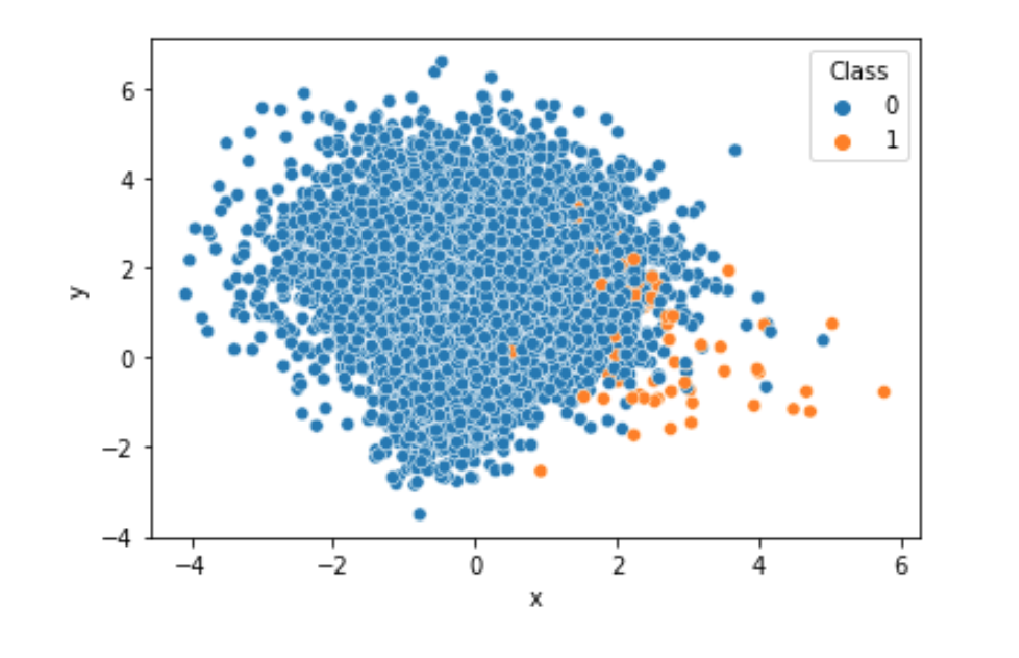
\includegraphics[scale=0.8]{image/data1.eps}
        \end{center}
    \end{figure*}
\end{center}

\subsection{German Credit Dataset}

The German Credit Dataset was downloaded from the UCI Machine Learning Repository, a web site that maintains many real datasets\cite{German}. 

The data set contains 1000 entries with 20 prepared category/symbol attributes
In this data set, each entry represents a person who receives credit from a bank. Each person is classified as a good or bad credit risk according to a set of attributes. We estimate it.
The data set is skewed with 700 out of 1000 entries for good credit risk.


\subsection{Haberman's Survival Data Set}

Haberman's Survival Data Set was similarly downloaded from the UCI Machine Learning Repository\cite{Haberman}.

The dataset contains case studies of survival of patients undergoing surgery for breast cancer conducted at the Billings Hospital of the University of Chicago between 1958 and 1970.
It has 306 data counts and three feature sets.
Estimate whether the patient died within 5 years.
It is a biased data set with 225 data that died within 5 years compared to 81 data that did not.

\subsection{Census-Income (KDD) Data Set}

The Census-Income (KDD) Data Set was similarly downloaded from the UCI Machine Learning Repository\cite{Census}.
This dataset contains weighted census data drawn from the 1994 and 1995 Current Population Surveys conducted by the U.S. Census Bureau. The data includes 41 demographic and employment related variables.
All categorical variables can be transformed into a Sparse One-Hot vector.
What we estimate is whether the income is greater than 50K or not.
We have a very large number of data, 32561, and the data is biased with 24720 being less than 50K.

\subsection{Blood Transfusion Service Center Data Set}

The Blood Transfusion Service Center Data Set was similarly downloaded from the UCI Machine Learning Repository\cite{Blood}.

This dataset contains data obtained from a blood transfusion service center located in Hsin Chu, Taiwan.
The center gives its blood transfusion service bus to one of the universities in Hsin Chu and collects donated blood about every three months. To build the marketing model which is a modified version of RFM, we randomly selected 748 donors from the donor database. For these 748 donor data, four variables were included. These are used to estimate whether a given donor has donated blood or not.

The data set is skewed, with 178 people who have donated blood compared to 570 who have not done so.
\clearpage


\section{Methods}
\subsection{SMOTE}

SMOTE is one method of random oversampling that increases the number of minority cases by randomly replicating the minority cases\cite{SMOTE}.

Below are the biased datasets.
Blue is the minority data set and orange is the majority data set.This can be seen in Fig. 2.2.

\begin{center}
    \begin{figure*}[ht]
        \caption{SMOTE: Before Oversampling.}
        \label{tab:team-rating-features}
        \begin{center}
            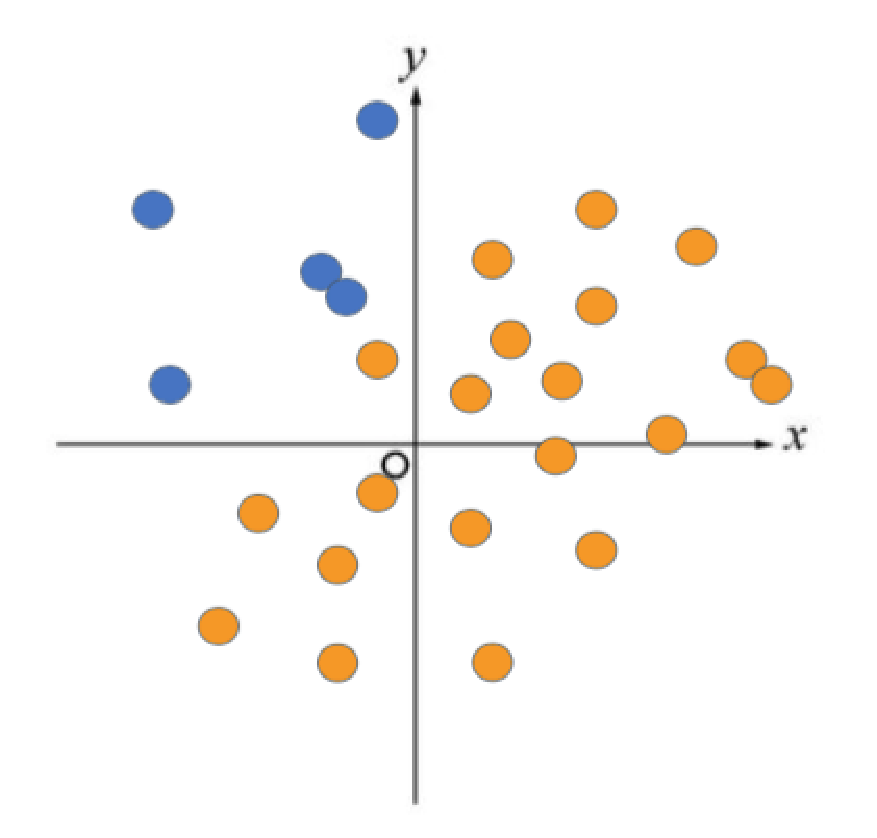
\includegraphics[scale=0.6]{image/smote1.eps}
        \end{center}
    \end{figure*}
\end{center}

\clearpage

Select one number group case. It's called $m_a$. This can be seen in Fig. 2.3.

\begin{center}
    \begin{figure*}[ht]
        \caption{SMOTE: Select a Case.}
        \label{tab:team-rating-features}
        \begin{center}
            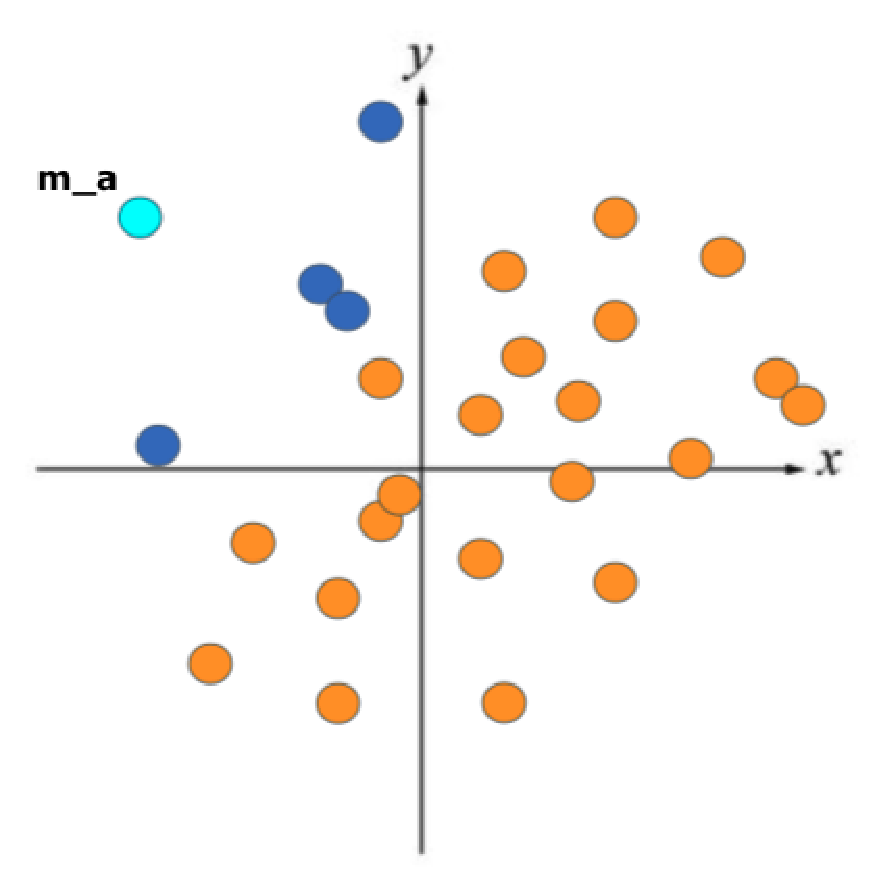
\includegraphics[scale=0.6]{image/smote2.eps}
        \end{center}
    \end{figure*}
\end{center}

\clearpage

Extract k data using the k-nearest neighbor method.
Calculate the degree of similarity between cases for a set of values of explanatory variables.
The similarity between vectors is calculated using the Euclidean distance

The j-th elements of $m_a$ and $m_i$ are written as $a_j$ and $i_j$, respectively.
$$
dis(m_a, m_i) = \Sigma_j(a_j - i_j)^2
$$
The figure below shows the k nearest neighbors painted in green. Figs2.4

\begin{center}
    \begin{figure*}[ht]
        \caption{SMOTE: Shows k nearest neighbor.}
        \label{tab:team-rating-features}
        \begin{center}
            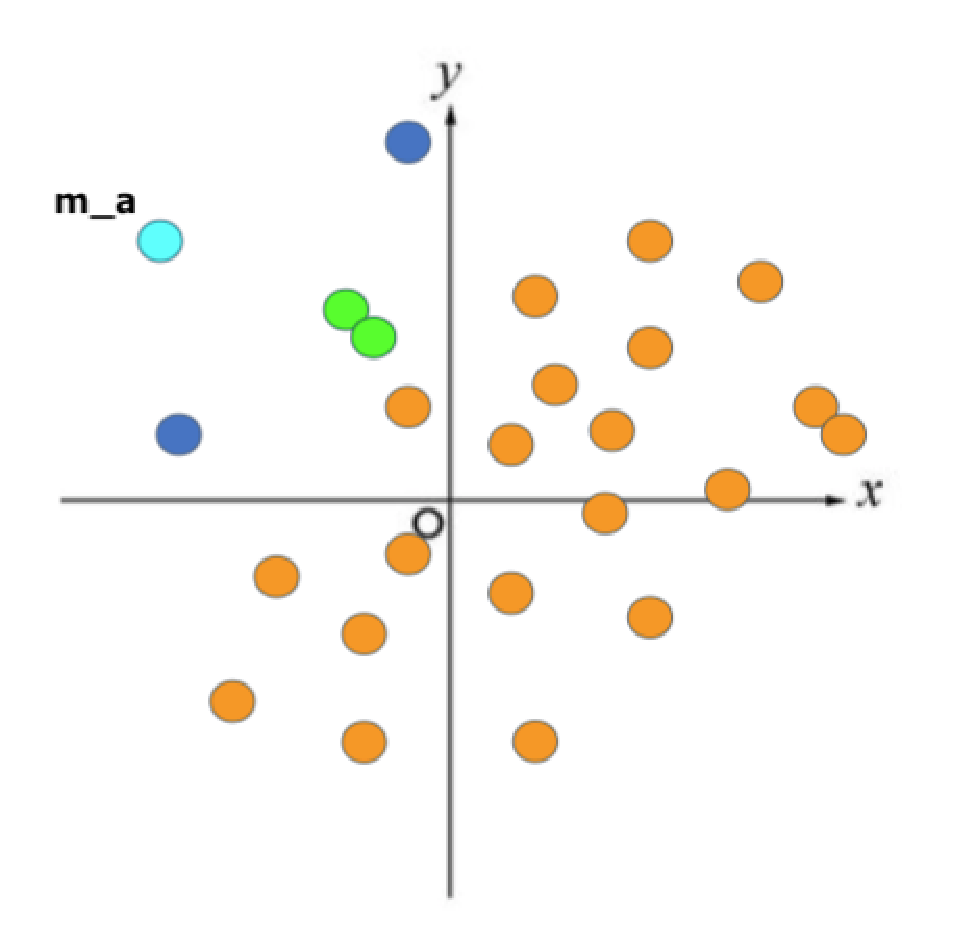
\includegraphics[scale=0.6]{image/smote3.eps}
        \end{center}
    \end{figure*}
\end{center}

\clearpage

Randomly select one of the k nearest neighbors.
In other words, pick one of the data that is colored green. Randomly.
I painted the selected one yellow.Figs2.5

\begin{center}
    \begin{figure*}[ht]
        \caption{SMOTE: Choose One Case from k nearest neighbors.}
        \label{tab:team-rating-features}
        \begin{center}
            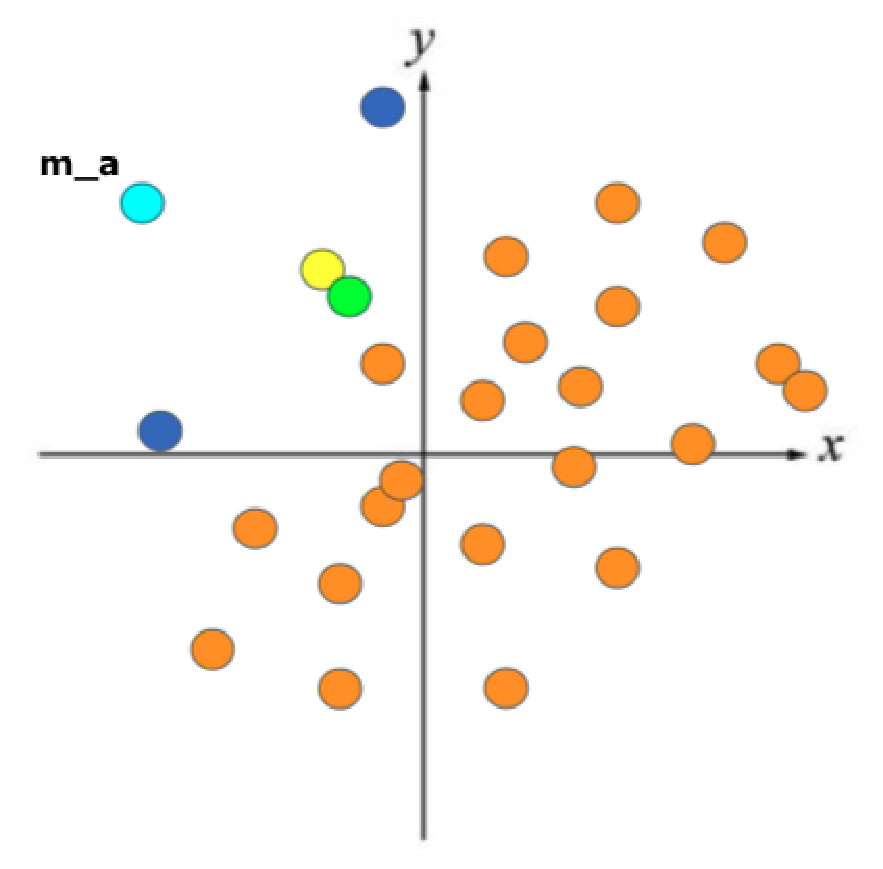
\includegraphics[scale=0.6]{image/smote4.eps}
        \end{center}
    \end{figure*}
\end{center}

\clearpage
Connect the first data you selected with the data you just selected with a straight line. Figs2.6.

\begin{center}
    \begin{figure*}[ht]
        \caption{SMOTE: Increase the number of new data in a linear fashion.}
        \label{tab:team-rating-features}
        \begin{center}
            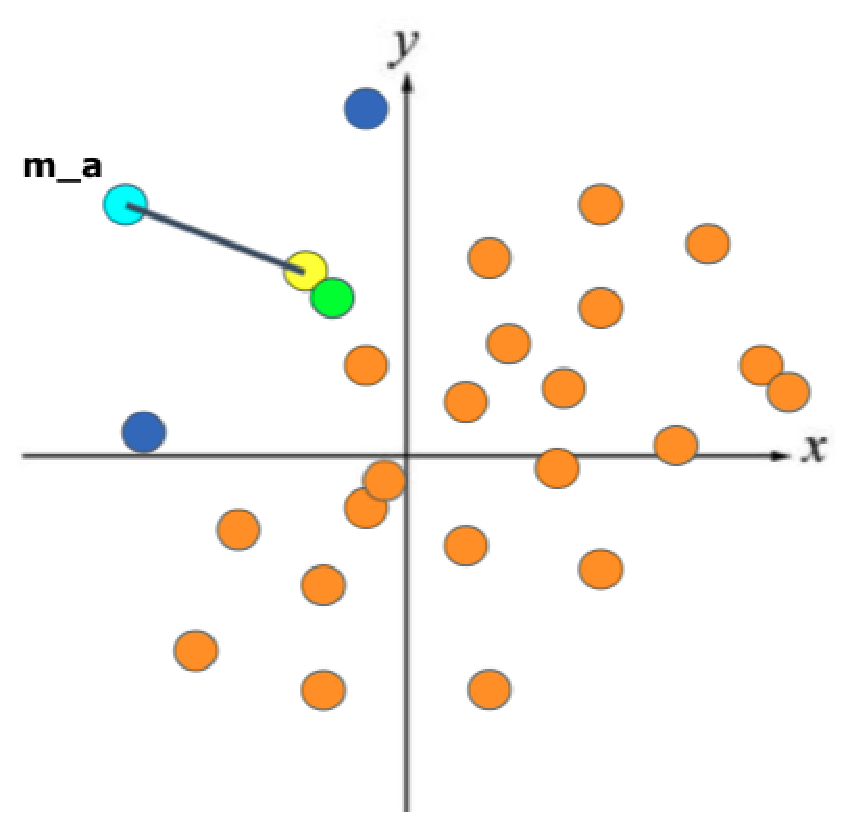
\includegraphics[scale=0.6]{image/smote5.eps}
        \end{center}
    \end{figure*}
\end{center}

It then generates some new data on that line.
This is the data that is generated by oversampling.
The position of the data on the line is completely random.

\clearpage
\subsection{Tomek-links}

One method of undersampling, which removes noisy samples, is to reduce the majority of the data set from a combination called Tomek Links\cite{TomekLinks}.

The algorithm is described below.
Below is a biased data set.
Blue is the minority data set and orange is the majority data set.

\begin{center}
    \begin{figure*}[ht]
        \caption{TOMEK-LINKS: Before undersampling dataset.}
        \label{tab:team-rating-features}
        \begin{center}
            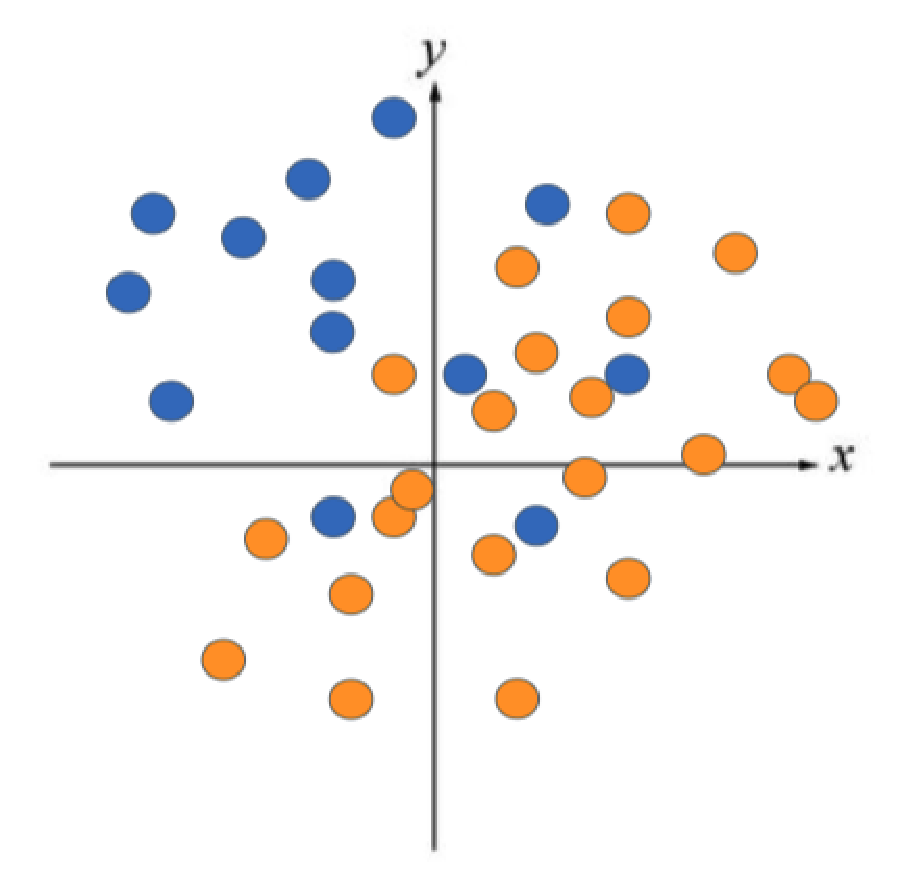
\includegraphics[scale=0.6]{image/tomek1.eps}
        \end{center}
    \end{figure*}
\end{center}

\clearpage

Tomek links are pairs of $x$ and $y$ such that there is no case $z$ in the dataset that satisfies $\delta(x, z) < \delta(x, y)$ or $\delta(y, z) < \delta(y, x)$.
However, we define $\delta(x, y)$ to be the distance between the minority case $x$ and the majority case $y$.

\begin{center}
    \begin{figure*}[ht]
        \caption{TOMEK-LINKS: Show the tomek-links.}
        \label{tab:team-rating-features}
        \begin{center}
            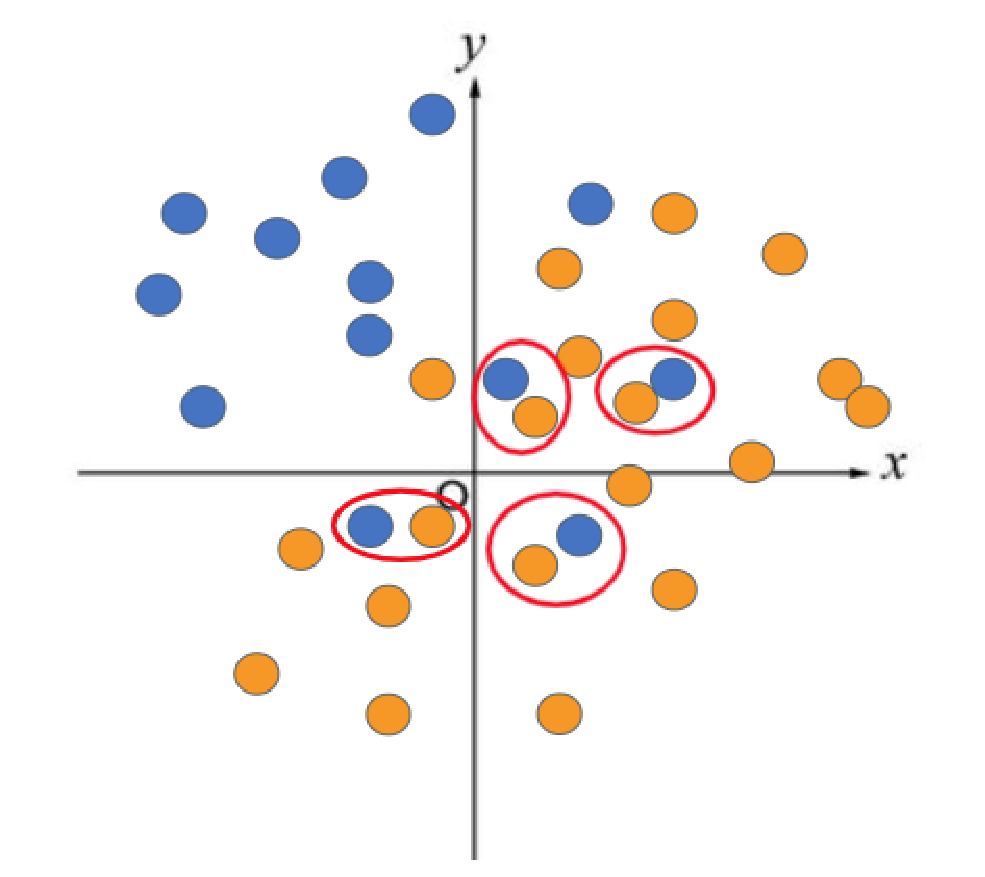
\includegraphics[scale=0.6]{image/tomek2.eps}
        \end{center}
    \end{figure*}
\end{center}

\clearpage

Delete the majority of data from these tomek links.

\begin{center}
    \begin{figure*}[ht]
        \caption{TOMEK-LINKS: Deleted tomek-links.}
        \label{tab:team-rating-features}
        \begin{center}
            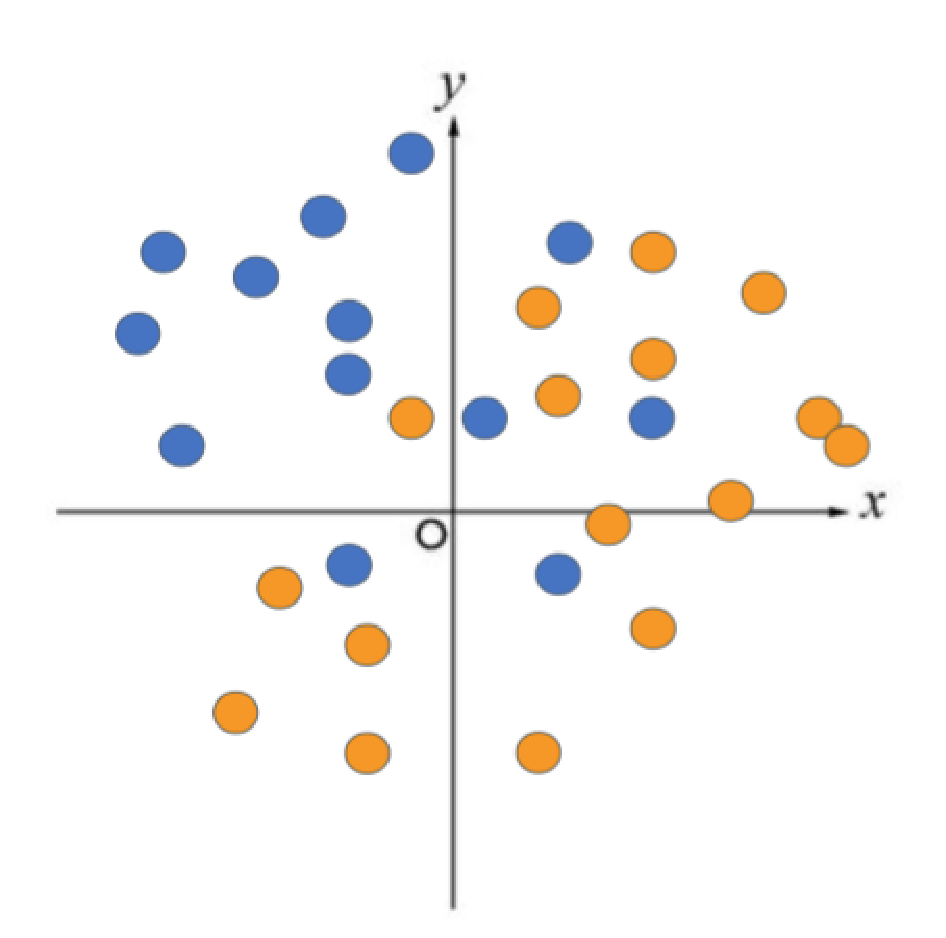
\includegraphics[scale=0.6]{image/tomek3.eps}
        \end{center}
    \end{figure*}
\end{center}

This process is repeated until there are no more two samples that are nearest neighbors of each other.
It prevents the majority from inferring that the training data has too much majority data, even if it has the characteristics of minority data.

\clearpage

\subsection{SMOTE + Tomek Combine}
In SMOTE + Tomek Combine, SMOTE and Tomek links are combined and over- and under-sampled.

\subsection{MySMOTE}

MySMOTE is an improved version of SMOTE.

Using a traditional SMOTE produces a linear data set.
In other words, linear data set is a straight line of data set
The boundaries between each class become blurred.
So, instead of sampling data on a straight line, I add noise and sampling data collectively.
The following is a description of the algorithm used by MySMOTE to perform oversampling.

\begin{center}
    \begin{figure*}[ht]
        \caption{MYSMOTE: How to calculate the noise.}
        \label{tab:team-rating-features}
        \begin{center}
            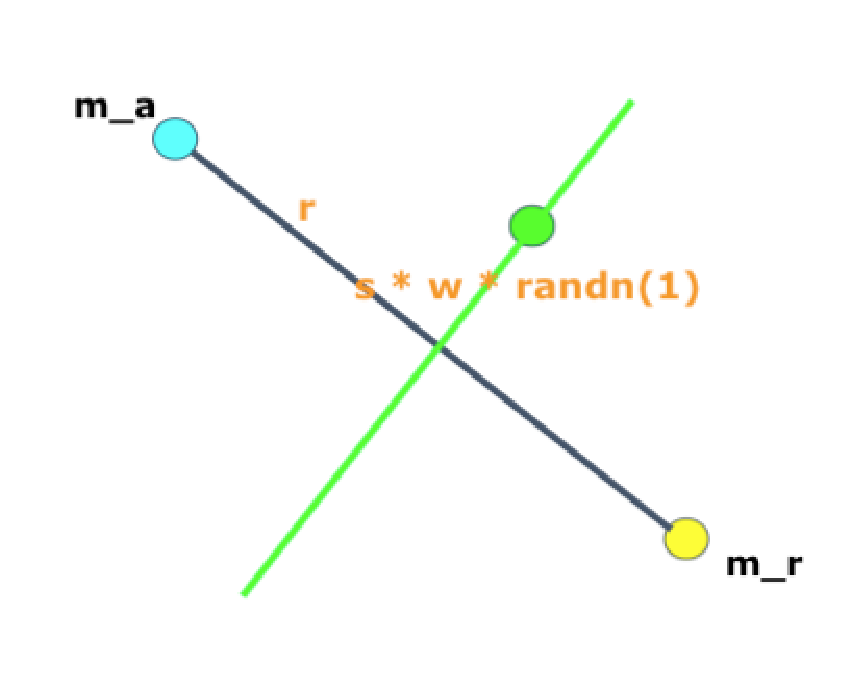
\includegraphics[scale=0.6]{image/mysmote1.eps}
        \end{center}
    \end{figure*}
\end{center}

Here is an explanation of the above variables.\\
$r$: This is a random value from $0$ to $1$ chosen uniformly.
This is the value used to determine the position of the new point generated between $m_a$ and $m_r$.
Noise is added to the point such that $m_a:m_r=r:1-r$, which is the new point.\\
$s$: Hyperparameter to determine how much noise to make.
The larger the value of $s$, the larger the noise will be.
The value range of $s$ is above 0.\\
$w$: This is the value of the variance of the explanatory variables.\\
I introduced it for the purpose of normalizing the magnitude of the noise to the explanatory variables.\\
$randn(1)$: randn outputs a random number with standard normal distribution.
The standard normal distribution is a Gaussian distribution with mean 0 and standard deviation 1.
This will randomly determine the size of the noise to be added.\\


Determine $m_a$ and $m_r$ as in SMOTE, and find the interior point such that $m_a:m_r=r:1-r$.
Up to this point, it is the same as SMOTE.
Then, the vector that is $s \times w \times randn(1)$ is called $\bm{v}$.
This $\bm{v}$ is noise.
Add $\bm{v}$ to the vector from the origin to its interior point.
In this way, we can now oversample not only the straight line connecting $m_a$ and $m_r$, but also the surrounding area.
By doing so, we aim to create a model that can determine the minority class for cases near the line connecting $m_a$ and $m_r$.

\section{What kind of model to experiment?}
As explained in the previous section, I train on a biased data set with some data preprocessing such as oversampling or undersampling.
I use scikit-learn to ensure that the learning is equal under all conditions. Decision Tree is used as the machine learning algorithm.
It is easy to think that decision trees are confusing when learning imbalanced data. This is because it removes branches that are considered to be too specialized and labels the new leaf nodes with the dominant class.
It becomes more likely that the majority class will become the dominant class of these leaf nodes, and it will not be able to capture the characteristics of the minority class.
To see if such a problem can be solved using oversampling or undersampling, a decision tree is used.
The details of the actual model used are as follows.

\begin{lstlisting}[caption=DecisionTreeClassifier,label=DecisionTreeClassifier]
sklearn.tree.DecisionTreeClassifier(*,
     criterion='gini',
     splitter='best',
     max_depth=3,
     min_samples_split=2,
     min_samples_leaf=1,
     min_weight_fraction_leaf=0.0,
     max_features=None,
     random_state=None,
     max_leaf_nodes=None,
     min_impurity_decrease=0.0,
     min_impurity_split=None,
     class_weight=None,
     ccp_alpha=0.0
)
\end{lstlisting}


\section{How to evaluate the model?}
A very commonly used evaluation metric for machine learning models is accuracy.
An index to determine how well the answer matches the overall prediction result. See below for the calculation formula.
$$
Accuracy = \frac{TP + TN}{TP + TN + FP + FN}
$$
And, $TP$ is the number of True Positive, $TN$ is the number of True Negative, $FP$ is the number of False Positive, and $FN$ is the number of False Negative cases. This section uses such an abbreviation.

Accuracy is an unreliable metric in imbalanced data.
This is because they can simply produce a high score.
For example, consfider a data set where 80 percent of the data is in the majority class and 20 percent in the minority class. If we have a model that labels all the data as majority class, the accuracy of the model will be 0.8.
This number is high, but it does not mean that this model is meaningless.
As the class distribution changes, so do these metrics, even if the performance of the underlying classifier does not change.
So it would be more interesting to use a performance metric that separates out the errors (or hits) that occur in each class.
In terms of these factors, I will use the AUC index\cite{ROC}.

The term AUC comes from Area Under the Curve.
The curve is the ROC curve, and the area of the lower right part is called the AUC.
And the ROC curve is a line graph in which the points corresponding to the vertical axis: true positive rate, and the horizontal axis: false positive rate, are plotted and connected for every $p$, assuming that "the estimated probability is greater than or equal to $p$ is considered positive.
Two more indicators will be introduced.
These are Precision and Recall.

Recall is a measure that refers to how many minority class cases were predicted without any oversights.
In other words, it is the percentage of minority class cases that are correctly determined to be minority class cases.
This is an important indicator when you want to ensure the success of your minority class inference.
$$
Recall = \frac{TP}{TP + FN}
$$
Precision is the percentage of patients predicted to be in the minority class that are really in the minority class.
In other words, it is the accuracy of the prediction of the minority class.
This indicator tends to decrease when you try to increase the Recall.
$$
Precision = \frac{TP}{TP + FP}
$$

\chapter{Results}

\section{What kind of model to experiment?}
As explained in the previous section, I train on a biased data set with some data preprocessing such as oversampling or undersampling.
I use scikit-learn to ensure that the learning is equal under all conditions. Decision Tree is used as the machine learning algorithm.
It is easy to think that decision trees are confusing when learning imbalanced data. This is because it removes branches that are considered to be too specialized and labels the new leaf nodes with the dominant class.
It becomes more likely that the majority class will become the dominant class of these leaf nodes, and it will not be able to capture the characteristics of the minority class.
To see if such a problem can be solved using oversampling or undersampling, a decision tree is used.
The details of the actual model used are as follows.

\begin{lstlisting}[caption=DecisionTreeClassifier,label=DecisionTreeClassifier]
sklearn.tree.DecisionTreeClassifier(*,
     criterion='gini',
     splitter='best',
     max_depth=3,
     min_samples_split=2,
     min_samples_leaf=1,
     min_weight_fraction_leaf=0.0,
     max_features=None,
     random_state=None,
     max_leaf_nodes=None,
     min_impurity_decrease=0.0,
     min_impurity_split=None,
     class_weight=None,
     ccp_alpha=0.0
)
\end{lstlisting}


\section{How to evaluate the model?}

Accuracy, or error rate, is an unreliable metric in imbalanced data.
This is because they can simply produce a high score.
For example, consfider a data set where 80 percent of the data is in the majority class and 20 percent in the minority class. If we have a model that labels all the data as majority class, the accuracy of the model will be 0.8.
This number is high, but it does not mean that this model is meaningless.
As the class distribution changes, so do these metrics, even if the performance of the underlying classifier does not change.
So it would be more interesting to use a performance metric that separates out the errors (or hits) that occur in each class.
In terms of these factors, I will use the AUC index\cite{ROC}.

\section{Results of various oversamplings and undersamplings}
This simple two-dimensional data can be visualized. The Results is following.

\clearpage

\subsection{Visualizing Simple 2D Data Set}
\subsubsection{Visualizing The Data Set}
Visualize a simple two-dimensional dataset that has been created.

\begin{center}
    \begin{figure*}[ht]
        \caption{Visualizing Simple 2D Data Set: Do Nothing Before Training}
        \label{tab:team-rating-features}
        \begin{center}
            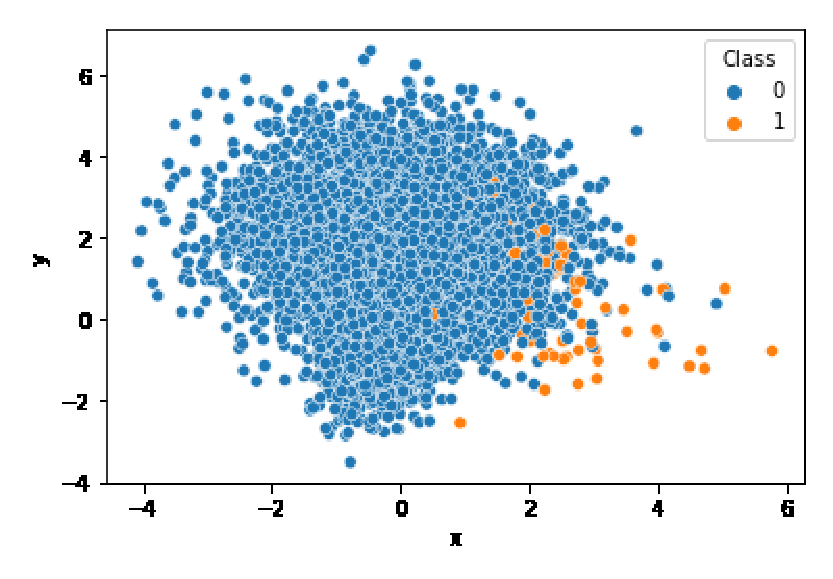
\includegraphics[scale=0.6]{image/no-prepro.eps}
        \end{center}
    \end{figure*}
\end{center}

\clearpage
\subsubsection{Visualizing Smote}
As a preprocessing step, using Smote, and the data set looked like this.

\begin{center}
    \begin{figure*}[ht]
        \caption{Visualizing Simple 2D Data Set: SMOTE}
        \label{tab:team-rating-features}
        \begin{center}
            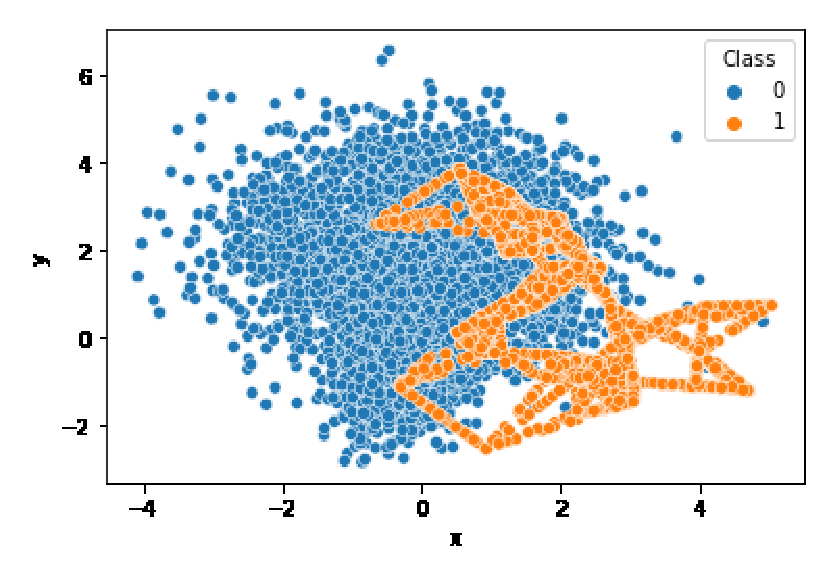
\includegraphics[scale=0.6]{image/smote.eps}
        \end{center}
    \end{figure*}
\end{center}
The linearly increasing data set shows the characteristics of the minority data.

\clearpage
\subsubsection{Visualizing Tomek Links}
Using undersampling with Tomek Links as preprocessing, the data set looked like this

\begin{center}
    \begin{figure*}[ht]
        \caption{Visualizing Simple 2D Data Set: Tomek Links}
        \label{tab:team-rating-features}
        \begin{center}
            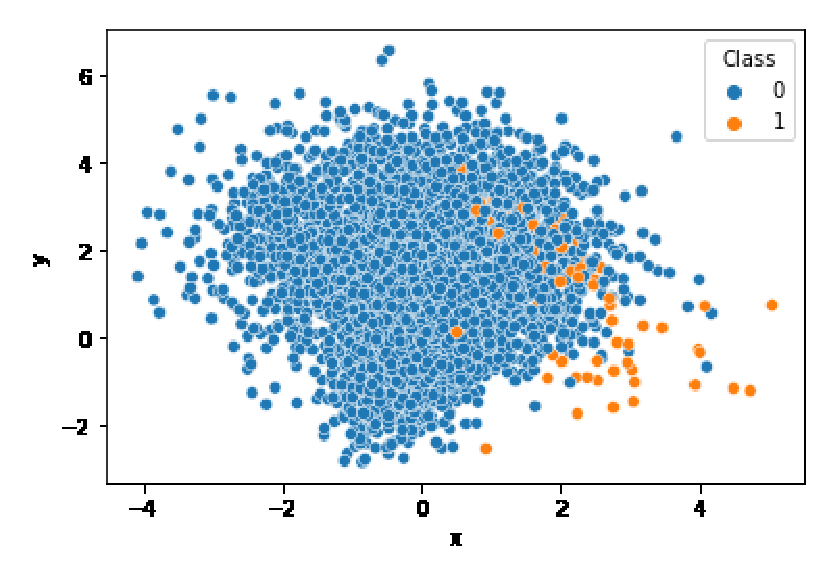
\includegraphics[scale=0.6]{image/tomek-links.eps}
        \end{center}
    \end{figure*}
\end{center}

I was not able to capture the features very effectively.
It may have been due to too much bias.

\clearpage
\subsubsection{Visualizing Smote and Tomek Links Combine}
With both Smote and undersampling using Tomek Links as preprocessing, the data set looked like this
\begin{center}
    \begin{figure*}[ht]
        \caption{Visualizing Simple 2D Data Set: Smote and Tomek Links Combine}
        \label{tab:team-rating-features}
        \begin{center}
            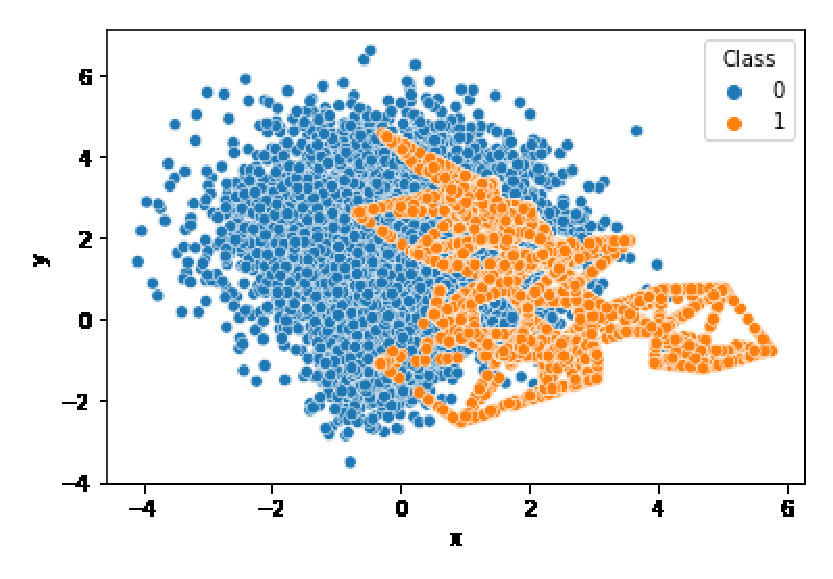
\includegraphics[scale=0.6]{image/combine.eps}
        \end{center}
    \end{figure*}
\end{center}
A few are strongly characterized by data that are not only linear.
It is thought that they appear more effectively when combined.

\clearpage
\subsubsection{Visualizing MySMOTE}
When using MySMOTE instead of Smote as preprocessing, the data set looked like this

\begin{center}
    \begin{figure*}[ht]
        \caption{Visualizing Simple 2D Data Set: MySMOTE}
        \label{tab:team-rating-features}
        \begin{center}
            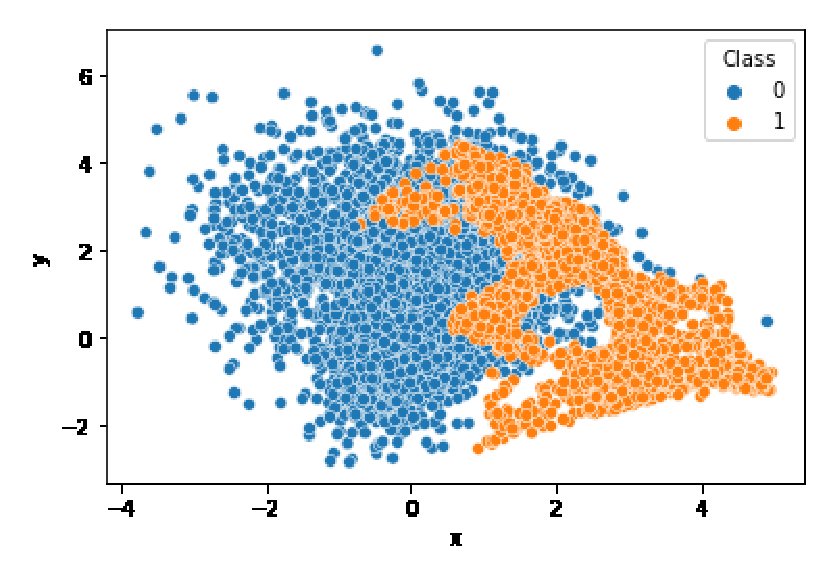
\includegraphics[scale=0.6]{image/mysmote.eps}
        \end{center}
    \end{figure*}
\end{center}

\clearpage

\subsection{The Table of Result}
\subsubsection{Simple 2D Data Set}
The actual results of adapting the model are shown below.
\begin{table}[H]
    \caption{Classification Result Simple 2D Dataset Table}
    \centering
    \begin{tabular}{|l|l|l|l|l|}
    \hline
         & Accuracy & precision & recall & AUC \\ \hline
        Without Pretreatment & 0.99100 & 0.6250 & 0.1724 & 0.58570 \\ \hline
        Using SMOTE & 0.92800 & 0.1055 & 0.8621 & 0.89536 \\ \hline
        Using Tomek-links & 0.99133 & 0.7143 & 0.1724 & 0.58587 \\ \hline
        Using Combine & 0.91500 & 0.0935 & 0.8966 & 0.90587 \\ \hline
        Using MySMOTE & 0.93233 & 0.1116 & 0.8621 & 0.89754 \\ \hline
    \end{tabular}
\end{table}


\subsubsection{German Credit Dataset}

\begin{table}[H]
    \caption{Classification Result German Credit Dataset}
    \centering
    \begin{tabular}{|l|l|l|l|l|}
    \hline
         & Accuracy & precision & recall & AUC \\ \hline
        Without Pretreatment & 0.68667 & 0.4500 & 0.5357 & 0.64054 \\ \hline
        Using SMOTE & 0.72333 & 0.5364 & 0.6484 & 0.70217 \\ \hline
        Using Tomek-links & 0.75000 & 0.6600 & 0.3626 & 0.64065 \\ \hline
        Using Combine & 0.68333 & 0.4861 & 0.7692 & 0.70758 \\ \hline
        Using MySMOTE & 0.63000 & 0.4026 & 0.7654 & 0.67267 \\ \hline
    \end{tabular}
\end{table}


\subsubsection{Haberman's Survival Data Set}

\begin{table}[H]
    \caption{Classification Result Haberman's Survival Dataset}
    \centering
    \begin{tabular}{|l|l|l|l|l|}
    \hline
         & Accuracy & precision & recall & AUC \\ \hline
        Without Pretreatment & 0.76087 & 0.6000 & 0.2500 & 0.59559 \\ \hline
        Using SMOTE & 0.59783 & 0.3488 & 0.6250 & 0.60662 \\ \hline
        Using Tomek-links & 0.76087 & 0.5556 & 0.4167 & 0.64951 \\ \hline
        Using Combine & 0.71739 & 0.4737 & 0.7500 & 0.72794 \\ \hline
        MySMOTE & 0.68478 & 0.4118 & 0.6087 & 0.65942 \\ \hline
    \end{tabular}
\end{table}

\subsubsection{Census-Income (KDD) Data Set}

\begin{table}[H]
    \caption{Classification Result Census-Income (KDD) Data Set}
    \centering
    \begin{tabular}{|l|l|l|l|l|}
    \hline
         & Accuracy & precision & recall & AUC \\ \hline
        Without Pretreatment & 0.84553 & 0.8618 & 0.9503 & 0.72808 \\ \hline
        Using SMOTE & 0.83816 & 0.8743 & 0.9206 & 0.74578 \\ \hline
        Using Tomek-links & 0.84553 & 0.8618 & 0.9503 & 0.72808 \\ \hline
        Using Combine & 0.73928 & 0.8948 & 0.7466 & 0.73109 \\ \hline
        MySMOTE & 0.84584 & 0.8624 & 0.9491 & 0.73248 \\ \hline
    \end{tabular}
\end{table}


\subsubsection{Blood Transfusion Service Center Data Set}

\begin{table}[H]
    \caption{Classification Result Blood Transfusion Service Center Data Set}
    \centering
    \begin{tabular}{|l|l|l|l|l|}
    \hline
         & Accuracy & precision & recall & AUC \\ \hline
        Without Pretreatment & 0.77778 & 0.6333 & 0.3276 & 0.63086 \\ \hline
        Using SMOTE & 0.74222 & 0.5000 & 0.4483 & 0.64629 \\ \hline
        Using Tomek-links & 0.77778 & 0.6333 & 0.3276 & 0.63086 \\ \hline
        Using Combine & 0.65333 & 0.4324 & 0.7619 & 0.68651 \\ \hline
        MySMOTE & 0.69333 & 0.4667 & 0.6667 & 0.68519 \\ \hline
    \end{tabular}
\end{table}


\chapter{Discussion}

The classification of disproportionate data is necessary in many situations.
For example, credit card fraud rates and positive rates of infectious diseases are extremely small percentages. It will become more and more common to use techniques such as machine learning and deep learning to solve these situations.

In this study, we first used a two-dimensional artificial data set that can be visualized. After that, we actually used four real datasets for learning and inference.
Then, we considered how to proceed with learning on imbalanced datasets in this study.
One of the problems in learning is that when the majority class and the minority class are treated as equals, it is nearly impossible to adequately grasp the characteristics of the minority class. In order to solve this problem, we considered the possibility of using oversampling and undersampling. 

In addition, it is difficult to evaluate the model when using imbalance data sets. Even if the percentage of correct answers is high, it may not be able to correctly discriminate the minority class. Therefore, in this study, we decided to judge whether the model is good or bad mainly by using the AUC value \cite{ROC}.

First, let's discuss the visualization of the Simple 2D Data Set. In this data set, it is easy to see that the orange class is the minority class. And since the minority data set is clustered on the right side, but the majority data set also appears on the right side, a normal adaptation of the model would probably give the majority class label to the cases on the right side as well. As we can see from the results, without any pretreatment, we could achieve very impressive results in the correct answer rate category. It was a whopping 0.99100. However, the recall score was only 0.1724. 
What this means is that only 10 percent of the cases from the minority class are predicted as members of the minority class. As mentioned earlier, this model almost completely ignores the minority data. As a result, it recorded a low AUC value, not commensurate with the percentage of correct answers. 

The solution to this problem was the oversampling method. We will refer to the visualization of oversampling using SMOTE. It can be seen that we have succeeded in representing the characteristics of the minority data. The characteristics are expressed in a very linear manner. This means that for the cases on this line, the model will give the minority label with confidence. Looking at the Table of Result, we can see that the results are as expected. The result is that the recall is now 0.8621 and the AUC has risen sharply to 0.89536. This is because we labeled the points on the line as minority class. Accuracy also dropped to 0.92800, but not drastically. Precision, however, was only 0.1055. This means that of those predicted to be in the minority, only 10\% of the cases actually belonged to the minority class. However, this is not a serious problem, because there are so few minority cases in this data set. The distribution was 99 vs. 1, which is a worthwhile oversampling because it is 10 times more accurate than a random response. 

The next step was to use Tomek Links. As you can see from the visualization, there is not much meaningful undersampling. I think this is because there are not enough minority data to make the class boundaries stand out in the undersampling. The results clearly showed this expectation, and the AUC values were very low. The next step was to use the Combine method. This is a method that further highlights the existence of minority classes by using both Smote and Tomek Links undersampling. The visualization shows that there are more cases from the minority class than in Smote. As a result, the recall increased further to 0.8966, and the AUC also increased accordingly to 0.90587.

Next, we conducted an experiment on MySMOTE, the proposed method of this study. The aim of MySMOTE is to capture the characteristics of the minority data not only linearly, which is a problem of SMOTE. We thought that this method, with the addition of noise, would be able to show the trend of minority data in a wider range. Let's take a look at the actual visualized data set. It is not just the linear increase in data that we have seen so far. We thought that we would be able to determine the boundary more strongly because there are many minority class data scattered around the data. However, as a score, recall was the same as before with Smote. In this dataset, the increased score due to the addition of noise did not seem to be of much use.

Next, we look at the table that shows the results of the German Credit Data Set. This is the result of using the first realistic data set. First, if we consider Smote, it increased the recall value significantly and raised the AUC significantly compared to the case where no oversampling or undersampling was used. This is similar to the simple two-dimensional data set described earlier. In addition, the precision was also increased by oversampling, which suggests that we have succeeded in grasping the features well. 

Next, when we consider Tomek Links, the results are the same as for the simple two-dimensional data set. However, in Combine with Smote, we were able to capture the features of the minority class more strongly than Smote, and the recall was further increased. However, the precision was reduced. As a result, the AUC value was almost zero. As a result, there was almost no change in the AUC value. 

Finally, the proposed method of this study, MySMOTE, was used. This method succeeded in increasing the recall significantly, as expected. However, due to the decrease in precision, the AUC was slightly lower than that of Smote and Combine. Although we were not able to improve the AUC itself, we were able to increase the recall more than Smote, so we were successful in labeling the minority class that did not ride in a linear fashion. However, the noise resulted in many of the majority classes being labeled as minority classes.

Next, we will refer to the table that shows the results of Haberman's Survival Data Set.
This table shows a slightly different result than the German Credit Data Set. First, let's consider Smote. There was no improvement in AUC. However, the recalls are definitely improved. Let's also consider Tomek Links. In this dataset, they have succeeded in improving the AUC. In the Haberman's Survival Data Set, we were able to capture the characteristics of the minority class by undersampling rather than oversampling. And when Combine is used, the AUC is dramatically improved.
Finally, there is MySMOTE, the proposed method of this study. MySMOTE, the proposed method of this study, was able to obtain higher AUC than that of Smote. However, it did not seem to work as well as Combine.

Next, we refer to the table that shows the results of the Census-Income (KDD) Data Set.
In this data set, the AUC did not change much by oversampling or undersampling. The reason is obvious: the value of recall is 0.9503 even without preprocessing, which is very high. The process of oversampling and undersampling is designed to work in favor of the minority classes. This is not an effective method for this data set since the aim is to increase the recall. 

Next, we refer to the table showing the results of the Blood Transfusion Service Center Data Set. This data set also shows very interesting results. The Smote and Tomek Links showed little improvement in AUC, but Combine and MySMOTE showed a large improvement in AUC. The improvement was not in precision, but in recall. This indicates that the linear oversampling of SMOTE did not identify many cases as minority class. Combining with undersampling and adding noise resulted in the correct identification of the minority class.


\chapter{Conclusion}

I used oversampling and undersampling techniques as an approach to learning from imbalanced data sets. In addition, I implemented a new oversampling method called MySMOTE.

What I found out strongly is that there is no silver bullet. Depending on the data set, the appropriate approach varies greatly. Even for Smote and Tomek Links, which one is superior or not depends on the data set. There were also cases where Combine worked well even when Smote and Tomek Links did not. Furthermore, Combine did not produce results that were less successful than Smote or Tomek Links. We felt that Combine is a very practical algorithm. 

MySMOTE, the proposed method in this thesis, was also found to work well on some datasets. When Smote or Tomek Links could not increase the recall, MySMOTE could greatly increase the recall and improve the AUC in some datasets. This suggests that MySMOTE may be a useful method for limited applications. 

Again, no silver bullet was found in the sampling method. We found that a more appropriate approach can be approached by considering not only results such as AUC, but also what specifically needs to be improved such as recall and precision, and taking various solutions into account.


% \input{problem_statement}
% \input{material}
% \input{evaluation}
% \input{result}
% \input{discussion}
% \input{conclusion}
%\chapter*{Acknowledgements}
%\addchapter{Acknowledgements}
\chapter*{Acknowledgements}
\addchapter{Acknowledgements}
I am grateful to Prof. Berrar for supporting my research and giving me comments and advice to improve my research.
I am also grateful to Prof. Uematsu, Prof. Matsuda, Prof. Matsumoto, and Prof. Jitsumatsu for their involvement in my research. 
Lastly, I would like to thank all the members of Berrar Lab for their support.

%\addchapter{References}
\addchapter{References}
\begin{thebibliography}{99}% 文献数が10未満の時 {9},10\UTF{FF5E}99の時 {99}

\bibitem{UCI}
``UCI Machine Learning Repository" \url{https://archive.ics.uci.edu/ml/index.php}.

\bibitem{German}
``UCI Machine Learning Repository, German Credit Data Set" \url{https://archive.ics.uci.edu/ml/datasets/statlog+(german+credit+data)}.

\bibitem{Haberman}
``UCI Machine Learning Repository, Haberman Data Set" \url{https://archive.ics.uci.edu/ml/datasets/haberman's+survival}.

\bibitem{Census}
``UCI Machine Learning Repository, Census Incom KDD Data Set" \url{https://archive.ics.uci.edu/ml/datasets/Census-Income+(KDD)}.

\bibitem{Blood}
``UCI Machine Learning Repository, Blood Transfusion Service Center Data Set" \url{https://archive.ics.uci.edu/ml/datasets/Blood+Transfusion+Service+Center}.

\bibitem{SMOTE}
``SMOTE" \url{https://imbalanced-learn.org/stable/references/generated/imblearn.over_sampling.SMOTE.html}.

\bibitem{TomekLinks}
``Tomek’s links" \url{https://imbalanced-learn.org/dev/references/generated/imblearn.under_sampling.TomekLinks.html}.

\bibitem{Combine}
``Combination of over- and under-sampling" \url{https://imbalanced-learn.org/dev/references/generated/imblearn.combine.SMOTETomek.html}.

\bibitem{ROC}
Shengping Yang PhD,
Gilbert Berdine MD,
``The receiver operating characteristic (ROC) curve," {\it The Southwest Respiratory and Critical Care Chronicles }, pp.34–36 2017

\bibitem{}
Gustavo E. A. P. A. Batista,
Ronaldo C. Prati,
Maria Carolina Monard,
``A study of the behavior of several methods for balancing machine learning training data" {\it ACM SIGKDD Explorations Newsletter},

\end{thebibliography}

\appendix\chapter{Source Code}
\label{appendix1}

The following Python code was what I used in this research.

\lstset{%
  language=Python,
  basicstyle={\ttfamily},
  breaklines=true,
  columns=[l]{fullflexible},
  lineskip=-0.5zw,
  frame=single,
}

\lstinputlisting[caption=without\_preprocessing.py,label=without-preprocessing]{../script/without_preprocessing.py}
\lstinputlisting[caption=smote.py,label=sote]{../script/smote.py}
\lstinputlisting[caption=tomek-links.py,label=tomek-links]{../script/tomek-links.py}
\lstinputlisting[caption=combine.py,label=combine]{../script/combine.py}
\lstinputlisting[caption=mysmote\_optuna.py,label=mysote-optuna]{../script/mysmote_optuna.py}
\lstinputlisting[caption=mysmote\_executer.py,label=mysmote-executer]{../script/mysmote_executer.py}
\lstinputlisting[caption=mysmote.py,label=mysote]{../script/mysmote.py}
\lstinputlisting[caption=simple\_2d.py,label=simple-2d]{../script/simple_2d.py}


% ----------------------------------------------------------------------
\end{document}
